\clearpage
\setcounter{page}{1}

\clearpage
% \onecolumn          % switch to full-width *before* supplementary

\appendix
% \suppressfloats[t]


\begin{center}
    \Large\bfseries Appendix
\end{center}
\vspace{1em}


\section{Implementation Details}
\label{sec:supp-impl}

This section provides implementation and evaluation details for the four video--action interaction programs studied in the main paper, including model architecture, downstream training, generation, and closed-loop evaluation.

\subsection{Model Architecture and Representation}
\label{sec:supp-architecture}

\paragraph{Dual-stream backbone.}
We use a 30-layer dual-stream Mixture-of-Transformers (MoT) architecture with modality-specific video and action experts.
The video expert has a hidden dimension of 3072, 24 attention heads with a head dimension of 128, and an FFN dimension of 14336. The action expert has a hidden dimension of 2048 and an FFN dimension of 8192, while retaining the same attention configuration of 24 heads with a head dimension of 128. Consequently, its query, key, and value projections each map the 2048-dimensional hidden state to 3072 dimensions, and the attention output is projected back to 2048 dimensions. 
Cross-modal information exchange is controlled by the future cross-modal attention pattern associated with each interaction program.
Task text conditions both streams through a separate cross-attention layer.

\paragraph{Visual observations.}
Each observation contains an agent-view image and a wrist-camera
image, both at $128\times128$ resolution. 
The two views are encoded independently into \(8\times8\times48\) VAE latents and concatenated along the spatial width dimension to form an \(8\times16\times48\) latent canvas.
Using a \(1\times2\times2\) temporal-spatial patch size, each latent frame contains 32 video tokens.
The video VAE temporally compresses every four environment steps into one latent video frame. Each generation chunk spans four future latent frames, corresponding to 16 environment steps.

\paragraph{Actions and proprioception.}
The policy predicts a 16-step action chunk aligned with the same temporal horizon, with four action steps corresponding to each latent video frame. Each action has seven dimensions: three for end-effector position, three for axis-angle rotation, and one for the gripper command. Each chunk is conditioned on an eight-dimensional proprioceptive state comprising the 3D end-effector position, a 3D axis-angle orientation converted from the simulator quaternion, and two gripper joint positions. The proprioceptive state is projected to the corresponding hidden dimension of each stream and added to its hidden representation rather than appended as a sequence token.

\subsection{Downstream Training}
\label{sec:supp-training}

The four interaction programs start from the same robot-video-pretrained causal backbone. The action expert is initialized from width-adapted copies of the corresponding pretrained video-expert layers, while action-specific input/output and conditioning layers are initialized separately. The video and action experts are then jointly optimized during downstream training. All programs use the same data, optimization settings, and flow-matching objective; they differ only in generation order and future cross-modal attention.

For the downstream runs examined here, training uses AdamW with
$\beta_1=0.9$, $\beta_2=0.95$, weight decay 0.1, a learning rate of
$10^{-5}$, with 10 warmup steps followed by a constant learning-rate schedule.
We use a per-device batch size of 1 and accumulate gradients over 10 steps, yielding an effective batch size of 10. Gradient norms
are clipped at 2.0, and training uses bf16 mixed precision.
We train all downstream models for 10,000 optimization steps. 
% All downstream models are trained on a single NVIDIA B200 GPU.

% \paragraph{Flow-matching objective.}
% Both streams are trained with a rectified-flow objective. Following
% the time convention used in the main text, a clean target $x_0$ and
% Gaussian noise $\epsilon$ define the interpolated input
% \begin{equation}
% x_{\tau}=(1-\tau)\epsilon+\tau x_0,
% \qquad
% u=x_0-\epsilon.
% \end{equation}
% Training times are sampled uniformly before the stream-specific
% noise schedules are applied. The video and action streams use
% separate noise schedules, with shift factors of 5.0 and 1.0,
% respectively. The flow-matching loss is applied to future video
% latents and valid action dimensions, with each modality normalized
% by its corresponding mask. Both losses use timestep-dependent
% weighting.
\paragraph{Flow-matching objective.}
Both streams are trained with the rectified-flow objective in
Eq.~(4). For implementation, we parameterize the noise level as
$\sigma = 1-\tau$, such that $\sigma=0$ denotes clean data and
$\sigma=1$ denotes pure noise. We uniformly sample from a
1,000-level base noise grid and apply the modality-specific shift
\begin{equation}
S_s(\sigma)
=
\frac{s\sigma}{1+(s-1)\sigma},
\qquad
s_V=5.0,\quad s_A=1.0,
\end{equation}
for video and action, respectively.

We additionally apply timestep-dependent loss weighting,
\begin{equation}
w_P(\sigma)
\propto
\exp\!\left[-2\left(\sigma-\tfrac{1}{2}\right)^2\right]
-
e^{-1/2},
\end{equation}
where the weights are normalized to have unit mean over the
corresponding timestep grid. This emphasizes intermediate noise
levels while assigning zero weight to the pure-noise endpoint.

The flow-matching loss is applied only to predicted future video
latents and valid action entries. Video losses are normalized over
the supervised latent elements, while action losses are averaged
over the action horizon after masking invalid action dimensions.
The two modality losses are combined with equal weight,
\begin{equation}
\mathcal{L}
=
\mathcal{L}_{V}
+
\mathcal{L}_{A}.
\end{equation}


\subsection{Video--Action Interaction Programs}
\label{sec:supp-programs}

The four programs differ in how predicted video and action
trajectories interact within a generation chunk. Each program
also receives the observed history and task instruction.

\paragraph{Joint.}
Video and action trajectories are denoised concurrently. During
generation, each stream can attend to the other stream's evolving
prediction, allowing bidirectional interaction before either
trajectory is complete.

\paragraph{Video-to-action (VTA).}
The model first generates the future video trajectory without
conditioning on future actions. It then generates the action
trajectory conditioned on the generated video trajectory.

\paragraph{Action-to-video (ATV).}
The model first generates the future action trajectory without
conditioning on future video. It then generates the video trajectory
conditioned on the generated action trajectory.

\paragraph{Decoupled.}
Video and action trajectories are generated concurrently, without
cross-modal interaction between their future predictions. Both
streams can still use the observed history and task instruction.

During training, the second stage of VTA and ATV conditions on the ground-truth trajectory of the first modality. 
At inference time, this ground-truth trajectory is replaced by the trajectory generated in the first stage. 
Joint and Decoupled jointly denoise both modalities in a single generation stage, whereas VTA and ATV use two sequential generation stages.

% \subsection{Inference and Closed-Loop Evaluation}
% \label{sec:supp-evaluation}

% \paragraph{Sampling.}
% Inference uses 20 denoising steps for video and 20 for actions with
% a UniPC solver. Video generation uses classifier-free guidance at
% scale 5.0; action generation uses a guidance scale of 1.0. Key--value
% caching is enabled. The inference attention window is 30 latent
% frames.

% \paragraph{Action execution.}
% By default, the policy executes the full predicted action chunk
% before replanning. Episodes are limited to 800 environment steps
% or 50 generated chunks. The rollout setup uses one model-observation
% frame at startup and five environment initialization steps.

% \paragraph{Evaluation protocol.}
% For each evaluated checkpoint, the recorded closed-loop protocol
% covers 10 tasks with 50 episodes per task. The episode index
% determines the environment seed, so programs evaluated under this
% protocol encounter the same set of initial conditions. Success is
% measured from the resulting environment rollouts.
\subsection{Inference and Closed-Loop Evaluation}
\label{sec:supp-evaluation}

\paragraph{Sampling.}
We use 20 denoising steps for each modality, with the same
modality-specific timestep schedules as in training. Video generation
uses classifier-free guidance with scale 5.0, while no classifier-free
guidance is applied to actions. Key--value caching is enabled during
inference. The history window spans 15 generation chunks, corresponding
to 60 latent video frames and the temporally aligned action history.

% \paragraph{Action execution.}
% The policy normally executes the full 16-step action chunk before
% replanning. For the first chunk, only 12 actions are executed because
% the first latent-frame group overlaps the startup observation. After
% resetting to the episode's initial state, the simulator is advanced for
% five zero-action steps to settle, and the policy is initialized from the
% final observation. Episodes terminate upon task success, after 800
% environment steps (including the five initialization steps), or after
% 50 generated chunks, whichever occurs first.
\paragraph{Action execution.}
After resetting to the episode's initial state, the simulator is advanced for
five zero-action steps to settle, and the policy is initialized from the final
observation. The first generation chunk conditions on this single observation;
the same startup convention is used during training, so no additional history
frames are required before the first prediction. The policy executes each
16-step action chunk before replanning. Episodes terminate upon task success,
after 800 environment steps (including the five initialization steps), or after
50 action chunks, whichever comes first.


% \paragraph{Evaluation protocol.}
% We evaluate each checkpoint on 10 tasks with 50 closed-loop episodes per
% task, for 500 episodes in total. Within each task, all interaction
% programs use the same 50 environment seeds and therefore share the same
% set of initial conditions. An episode is counted as successful if the
% simulator's task-success predicate is satisfied at any environment step,
% at which point the rollout terminates. We report the mean success rate
% over the 500 episodes.
\paragraph{Evaluation protocol.}
For each interaction program, we evaluate three independently trained
seeds. Each checkpoint is evaluated on 10 tasks with 50 closed-loop
episodes per task, for 500 episodes per seed. Within each task, all
interaction programs use the same 50 environment seeds and therefore
share the same set of initial conditions. An episode is counted as
successful if the simulator's task-success predicate is satisfied at
any environment step, at which point the rollout terminates. We report
the mean and standard deviation of the success rate across the three seeds.

\subsection{Real Robot Setup}

\begin{figure}[t]
    \centering
    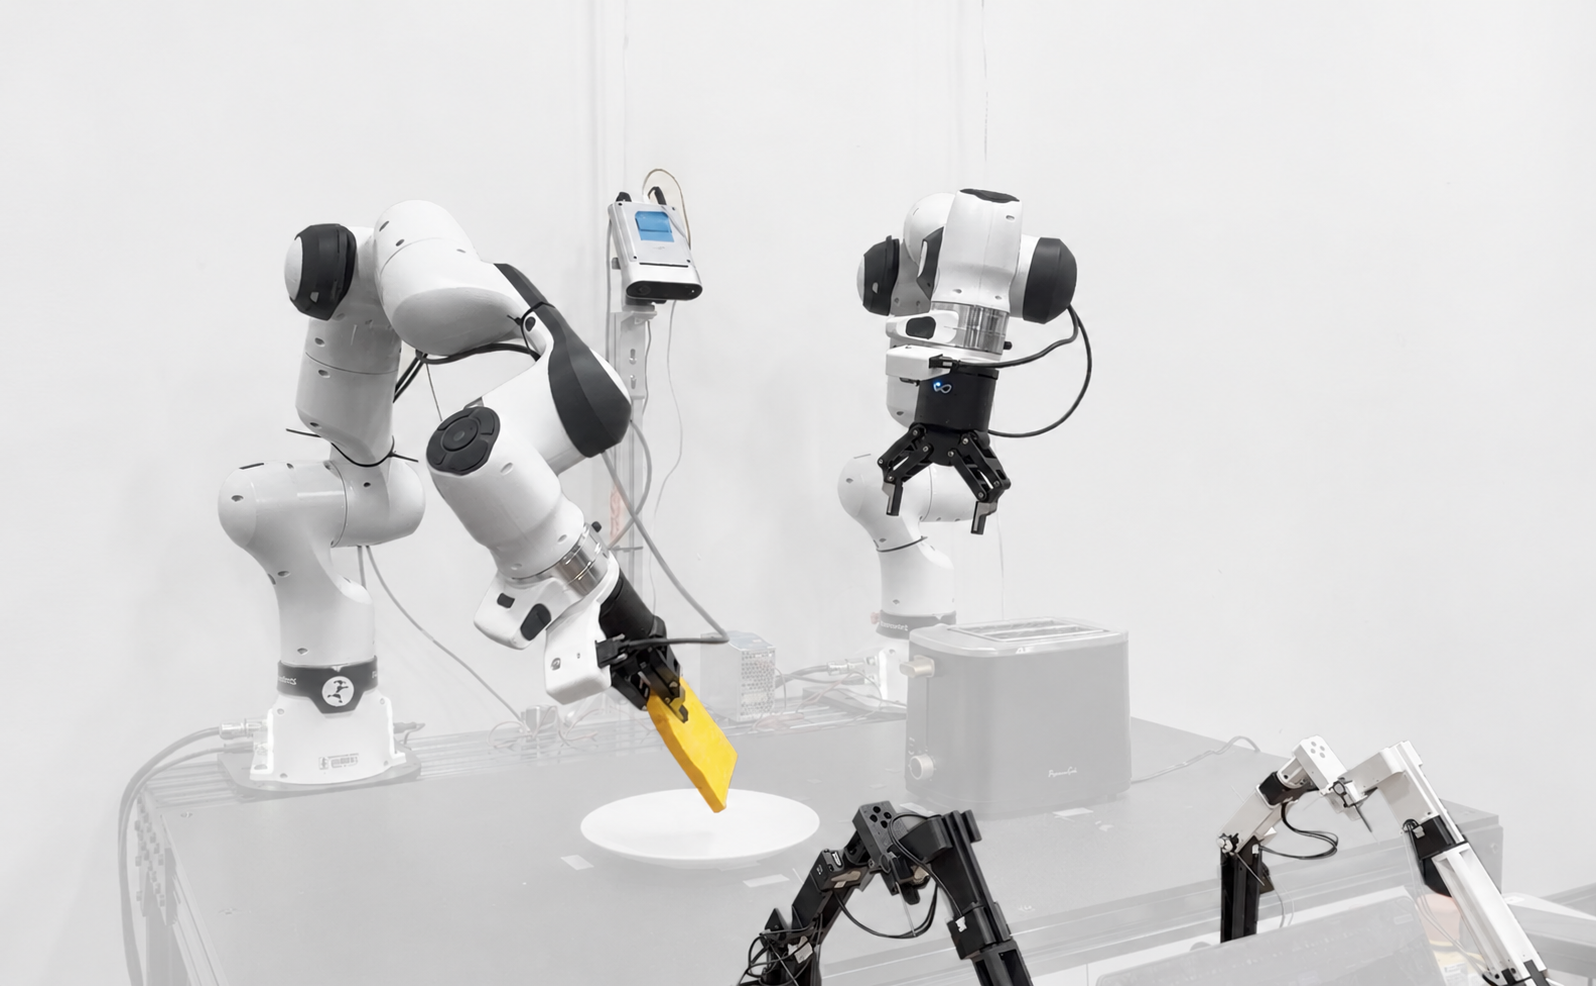
\includegraphics[width=0.98\linewidth]{sec/images/openwam-real-setup.png}
    \caption{Real-world bimanual setup with two Franka FR3 arms, Flexiv Grav grippers, bimanual GELLO teleoperation~\cite{wu2024gello}, two wrist-mounted RealSense D405 cameras, and a central Orbbec Femto Mega camera.}
\label{fig:real_robot_setup}
\end{figure}

The real-robot setup, as shown in Figure~\ref{fig:real_robot_setup}, consists of two Franka FR3 arms with Flexiv Grav grippers. We collect demonstrations through bimanual GELLO teleoperation. Two wrist-mounted RealSense D405 cameras record at 1280 × 720 pixels, and a central Orbbec Femto Mega records at 1920 × 1080 pixels, all at 30 fps. Joint positions, end-effector poses, gripper widths, and control commands are recorded with timestamps at 30 Hz. In the chunk-relative formulation, each arm’s target poses are expressed relative to its observed pose at the start of the chunk, while gripper widths remain absolute. Each action contains 20 values: three position coordinates, six values representing orientation, and one gripper width for each arm.

For the real-robot experiments, we collect 200 demonstrations each for
Toast Bread and Rubik's Cube, and 180 demonstrations for Sort Cups.
Each demonstration is 30\,s long. We evaluate the learned
policies over 50 closed-loop episodes for Toast Bread and Rubik's Cube,
and 36 episodes for Sort Cups.




\begin{table*}[t]
    \centering
    \caption{
    Data used for causal robot-video pretraining. 
    }
    \label{tab:pretraining-corpus}
    \small
    \begin{tabular}{@{}lrrl@{}}
        \toprule
        \textbf{Dataset}
        & \textbf{Trajectories / takes}
        & \textbf{Hours}
        & \textbf{Source type} \\
        \midrule

        Open X-Embodiment (49 manipulation datasets)
        & 1,300,749
        & 1,911.29
        & Multi-embodiment robot data \\

        AgiBot World Beta
        & 1,003,672
        & 2,976.4
        & Real robot manipulation \\

        Ego-Exo4D v2
        & 5,035
        & 221.26
        & Human interaction \\

        InternData-A1
        & 637,498
        & 7,433.91
        & Synthetic robot manipulation \\

        RoboCOIN
        & 183,157
        & 1,306.83
        & Real bimanual manipulation \\

        RoboMIND
        & 107,877
        & 305.5
        & Multi-embodiment robot data \\

        FastUMI-100K
        & 92,823
        & 461.77
        & Human-guided manipulation \\

        UMI family
        & 5,430
        & 24.60
        & Human-guided manipulation \\

        \bottomrule
    \end{tabular}
\end{table*}

\section{Robot-Video Pretraining}
\label{app:video-pretraining}

We adapt the Wan2.2-5B video backbone to robot-centric motion and physical
interaction before introducing action prediction. The pretraining corpus
combines robot demonstrations, human manipulation video, and synthetic robot
trajectories across a broad range of embodiments, viewpoints, objects, and
interaction patterns. No action labels are used during this stage.

\subsection{Pretraining Corpus}
\label{app:pretraining-data}

Our robot-video pretraining corpus combines large-scale real-robot manipulation,
human interaction video, and synthetic robot trajectories. Table~\ref{tab:pretraining-corpus}
summarizes the source data before training-window sampling. The UMI-family entry
aggregates UMI, DexUMI~\cite{xu2025dexumi}, UMI on Legs~\cite{ha2024umilegs}, and MV-UMI.

The corpus contains approximately 3.34 million trajectory or take units and
14.64k nominal hours, spanning heterogeneous robot embodiments, collection
interfaces, viewpoints, human-object interactions, and synthetic manipulation
at scale, providing the visual and interaction prior used by all downstream
\ours models.


\subsection{Causal Adaptation}
\label{app:pretraining-causal}

Pretraining starts from the Wan2.2-5B checkpoint. We retain the pretrained
video representation and optimize the model on the corpus above using the
chunk-causal prediction objective described in Sec.~\ref{sec:method}. Future
chunks may attend to the current observation, preceding observations, and
previously generated chunks, but not to later chunks. Tokens within each
chunk are denoised jointly.

This stage uses video alone. Robot actions, proprioception, and task-specific
policy targets are not supplied to the model. The resulting checkpoint serves
both as a standalone causal video predictor and as the common visual
initialization for the downstream \ours interaction programs.

\subsection{Training Compute}
\label{app:pretraining-compute}

Causal robot-video pretraining is performed on 32 NVIDIA B200 GPUs for
14 days. All downstream \ours variants in the main experiments start from
the resulting checkpoint unless otherwise specified.



\section{LIBERO-Long-CF: Counterfactual Dynamics Data}
\label{app:libero-cf}

LIBERO demonstrations contain task-directed behavior and cover only a small
fraction of the local state--action--outcome distribution. From each visited
state, they provide essentially one successful action continuation. This is
well suited to imitation learning but provides limited supervision for inverse
and forward dynamics, which must model how alternative actions correspond to
alternative physical outcomes.

We construct \textbf{LIBERO-Long-CF} by branching from task-relevant states in
the ten LIBERO-Long tasks and executing modified future action sequences.
The dataset contains 32,000 counterfactual segments, balanced across tasks.
Each segment contains 128 future controls and 129 synchronized two-view
observations. The original tasks, assets, and simulator physics are preserved.

\subsection{Scale and Intervention Coverage}
\label{app:libero-cf-scale}

LIBERO-Long-CF contains 4.10 million control records, compared with 138,090
controls in the 500 source demonstrations, increasing local transition
supervision by approximately $29.7\times$. At 20\,Hz, these correspond to
56.9 and 1.92 control-equivalent hours, respectively.

\begin{table}[t]
    \centering
    \caption{
    Scale of LIBERO-Long-CF and the source LIBERO-Long demonstration corpus.
    }
    \label{tab:libero-cf-scale}
    \small
    \begin{tabular}{@{}lcc@{}}
        \toprule
        \textbf{Quantity}
        & \textbf{Demonstrations}
        & \textbf{LIBERO-Long-CF} \\
        \midrule
        Tasks
        & 10
        & 10 \\
        Stored sequences
        & 500
        & 32,000 \\
        Sequences / task
        & 50
        & 3,200 \\
        Controls / sequence
        & 276.2 mean
        & 128 \\
        Total controls
        & 138,090
        & 4,096,000 \\
        Duration
        & 1.92 h
        & 56.9 h \\
        \bottomrule
    \end{tabular}
\end{table}

The branch generator modifies motion magnitude, direction, temporal structure,
individual action axes, stochastic arm motion, and gripper behavior.
Table~\ref{tab:libero-cf-composition} summarizes the intervention distribution.

\begin{table}[t]
    \centering
    \caption{
    Intervention composition of LIBERO-Long-CF. Categories denote generation
    recipes and may induce overlapping physical effects.
    }
    \label{tab:libero-cf-composition}
    \small
    \begin{tabular}{@{}lr@{}}
        \toprule
        \textbf{Intervention family}
        & \textbf{Fraction (\%)} \\
        \midrule
        Stop / rescale arm motion
        & 9.4 \\
        Reverse / redirect translation
        & 6.3 \\
        Axis biases and pulses
        & 12.5 \\
        Dedicated yaw perturbation
        & 3.1 \\
        Noise / randomized arm controls
        & 12.5 \\
        Dedicated gripper interventions
        & 31.3 \\
        Random-duration arm / gripper interventions
        & 25.0 \\
        \bottomrule
    \end{tabular}
\end{table}

Interventions include stopped and rescaled motion, reversed or redirected
translation, translational and rotational pulses, structured control noise,
piecewise-random commands, and changes to gripper state and timing. All
commands are within LIBERO's normalized controller range.

\subsection{State and Interaction Coverage}
\label{app:libero-cf-coverage}

Within the dataset, 75\% of segments begin from demonstration-prefix states.
The remaining 25\% begin after an additional executed perturbation, extending
the starting-state distribution beyond the demonstrated trajectories.

Among characterized perturbed starts, the end-effector state is on average
3.34\,cm from the nearest point on the corresponding demonstrated path
(median 1.90\,cm). Under thresholds of 1\,cm translation, $5^\circ$ rotation,
or 5\% articulated-joint travel, 61.6\% also contain object configurations
outside the corresponding demonstrated configurations.

The corpus contains substantial physical interaction. As shown in
Table~\ref{tab:libero-cf-interaction}, 90.4\% of characterized segments contain
gripper contact with an object or fixture, 50.0\% contain a detected grasp,
and 72.3\% alter object configuration relative to the same-start reference
continuation.

\begin{table}[t]
    \centering
    \caption{
    Physical interaction statistics for LIBERO-Long-CF. Categories overlap.
    }
    \label{tab:libero-cf-interaction}
    \small
    \begin{tabular}{@{}lr@{}}
        \toprule
        \textbf{Measured interaction}
        & \textbf{Rate (\%)} \\
        \midrule
        Gripper--object / fixture contact
        & 90.4 \\
        Detected grasp
        & 50.0 \\
        Object-configuration effect
        & 72.3 \\
        \bottomrule
    \end{tabular}
\end{table}

\subsection{Representation for Local Dynamics Learning}
\label{app:libero-cf-representation}

Each segment contains two synchronized $128\times128$ RGB streams,
128 seven-dimensional delta-OSC controls, and 129 proprioceptive states.
Actions contain three translation channels, three rotation channels, and one
gripper command.

Both camera streams are encoded with the \ours video VAE. The encoded
sequence contains one boundary observation and 32 future latent frames, with
four controls aligned to each future latent frame.

Local-context IDM conditions on the boundary observation, proprioception, and
future visual trajectory to predict the action sequence. Local-context FDM
conditions on the boundary observation, proprioception, and action sequence to
predict the future visual trajectory. Both objectives exclude task language
and pre-start history.

 

\section{Ablations}
\subsection{Effect of Video-Backbone Initialization}
\label{app:init-ablation}
We further examine whether the benefit of robot-video pretraining is specific to
VTA or persists across interaction programs. Under otherwise matched downstream
training, we initialize the video backbone either randomly, from the original
Wan2.2 checkpoint, or from our robot-video-pretrained causal checkpoint.
Table~\ref{tab:init-program-ablation} shows a consistent ordering for both VTA
and Joint. Relative to Wan2.2 initialization, robot-video pretraining improves
success by 29.4 percentage points for VTA and 34.4 points for Joint, reaching
97.8\% and 96.6\%, respectively. Random initialization performs substantially
worse for both programs. These results indicate that the benefit of the
robot-video-pretrained backbone transfers across distinct video--action interaction
structures.

\begin{table}[t]
    \centering
    \caption{
    Effect of video-backbone initialization on closed-loop LIBERO-Long success.
    Downstream architecture and training are held fixed within each interaction
    program.
    }
    \label{tab:init-program-ablation}
    \small
    \begin{tabular}{@{}lcc@{}}
        \toprule
        \textbf{Video initialization}
        & \textbf{VTA (\%)}
        & \textbf{Joint (\%)} \\
        \midrule
        Random initialization
        & 20.0
        & 27.2 \\
        Original Wan2.2
        & 68.4
        & 62.2 \\
        Robot-video pretrained
        & \textbf{97.8}
        & \textbf{96.6} \\
        \bottomrule
    \end{tabular}
\end{table}



\begin{table}[t]
    \centering
    \caption{
    Effect of the Mixture-of-Transformers architecture on closed-loop
    LIBERO-Long success. All variants use robot-video-pretrained
    initialization.
    }
    \label{tab:mot-ablation}
    \small
    \begin{tabular}{@{}lcc@{}}
        \toprule
        \textbf{Architecture}
        & \textbf{VTA (\%)}
        & \textbf{Joint (\%)} \\
        \midrule
        Non-MoT
        & 92.8
        & 93.6 \\
        MoT
        & \textbf{97.8}
        & \textbf{96.6} \\
        \bottomrule
    \end{tabular}
\end{table}


\begin{table*}[t]
    \centering
    \caption{
    Policy and dynamics accuracy on LIBERO-Long.
    LC-IDM and LC-FDM are independently trained specialist checkpoints;
    the multi-objective model trains policy, IDM, and FDM within a single
    checkpoint. 
    Lower is better for MSE and IDM error; higher is better for success and SSIM.
    }
    \label{tab:external-dynamics}
    \scriptsize
    \setlength{\tabcolsep}{3.2pt}
    \resizebox{\textwidth}{!}{
    \begin{tabular}{@{}l
        c
        cccc
        cccc@{}}
        \toprule
        &
        \textbf{Policy}
        &
        \multicolumn{4}{c}{\textbf{Real demonstrations}}
        &
        \multicolumn{4}{c}{\textbf{Counterfactual transitions}} \\
        \cmidrule(lr){2-2}
        \cmidrule(lr){3-6}
        \cmidrule(lr){7-10}

        \textbf{Model}
        & \textbf{Succ. (\%)}
        & \textbf{FDM MSE $\downarrow$}
        & \textbf{FDM SSIM $\uparrow$}
        & \textbf{IDM pos. (cm) $\downarrow$}
        & \textbf{IDM rot. ($^\circ$) $\downarrow$}
        & \textbf{FDM MSE $\downarrow$}
        & \textbf{FDM SSIM $\uparrow$}
        & \textbf{IDM pos. (cm) $\downarrow$}
        & \textbf{IDM rot. ($^\circ$) $\downarrow$} \\
        \midrule

        \ours, LC-IDM, CF-only
        & --
        & --
        & --
        & 1.76
        & 2.39
        & --
        & --
        & \textbf{1.17}
        & 3.60 \\

        \ours, LC-IDM, mixed
        & --
        & --
        & --
        & 0.44
        & 1.21
        & --
        & --
        & 1.22
        & 3.68 \\

        \ours, LC-FDM, CF-only
        & --
        & 0.00734
        & 0.9126
        & --
        & --
        & \textbf{0.00940}
        & \textbf{0.8889}
        & --
        & -- \\

        \ours, LC-FDM, mixed
        & --
        & 0.00186
        & 0.9776
        & --
        & --
        & 0.00962
        & 0.8859
        & --
        & -- \\

        \midrule

        \ours, multi-objective
        & \textbf{92.8}
        & \textbf{0.00058}
        & \textbf{0.9934}
        & \textbf{0.43}
        & \textbf{1.10}
        & 0.01416
        & 0.8398
        & 1.73
        & \textbf{3.55} \\

        UVA
        & 88.0
        & 0.00279
        & 0.9645
        & 2.03
        & 1.60
        & 0.01514
        & 0.8134
        & 3.57
        & 12.99 \\

        \bottomrule
    \end{tabular}
    }
\end{table*}


\subsection{Effect of the Mixture-of-Transformers Architecture}
\label{app:mot-ablation}

We isolate the effect of the Mixture-of-Transformers (MoT) parameterization
while keeping the pretrained visual foundation fixed. Both variants start
from the same robot-video-pretrained video checkpoint and use the same
downstream data and training procedure. In the non-MoT variant, video and
action tokens are processed by the same pretrained DiT; the MoT variant retains the pretrained video expert and introduces a separate action expert initialized from width-adapted copies of the corresponding video-expert layers. As shown in Table~\ref{tab:mot-ablation}, the
shared-DiT model already achieves strong performance, reaching 92.8\% for
VTA and 93.6\% for Joint. MoT further improves success to 97.8\% and
96.6\%, corresponding to gains of 5.0 and 3.0 percentage points,
respectively. 

\section{External Dynamics Comparison}
\label{app:external-dynamics}

We compare \ours with UVA~\cite{li2503unified}, the closest released
LIBERO system in our related work that exposes policy, inverse-dynamics,
and forward-dynamics objectives within one model. Table~\ref{tab:external-dynamics}
covers two settings: independently trained local-context dynamics components
and a single multi-objective checkpoint trained jointly across policy, IDM,
and FDM objectives.

For FDM, we report RGB prediction error in a common agent-view image space.
For IDM, the two systems use different action parameterizations, so we compare
the resulting end-effector trajectory error after executing the predicted
actions from the same simulator state.

\subsection{Independent Dynamics Components}

The LC-IDM and LC-FDM specialists are trained either on counterfactual
transitions only or on a 60/40 mixture of counterfactual and demonstration
transitions. CF-only specialists are strongest on the held-out
counterfactual distribution, while mixed supervision substantially improves
fidelity on real demonstrations. Both remain well ahead of UVA on the
counterfactual dynamics metrics.

\newpage

\subsection{Unified Policy and Dynamics Modeling}

UVA trains policy generation, inverse dynamics, and forward dynamics within a
single model. We therefore also evaluate one \ours checkpoint trained with
60\% real joint video--action supervision, 20\% local-context IDM supervision,
and 20\% local-context FDM supervision; the IDM and FDM portions are each split
equally between demonstration and counterfactual transitions.

The unified \ours checkpoint outperforms UVA on policy success and on the
evaluated IDM and FDM metrics. Its counterfactual dynamics accuracy is weaker
than that of the dedicated specialists, showing the expected tradeoff between
multi-objective training and specialization. The unified \ours checkpoint also gives the lowest IDM and FDM errors on real
demonstrations. These numbers measure fit to the demonstration distribution,
not held-out generalization, because some of the same demonstrations may also
be seen by the policy objective during training. Its policy score is also lower
than the policy-specialized \ours models as only 60\% of training updates
optimize the policy objective.


